\section{\textbf{Our Approach}}\label{sec:main}
\subsection{ Proposed Solution}

Based on the demand of the project we decided to use
Plug-in feature of WordPress since there were so many other
options like using the timeline feature of MPAT or developing
an application by using Multi-sites and a separate database.
etc. WordPress plugin is a piece of software written in PHP
that contains different functions and features to extend the
functionality of the WordPress environment, and it does not
change anything in the core functionality of WordPress. Plugins
functionality can be very elastic, and it can be simple like
just printing Hello World, or complex as plugins like Yoast
SEO for WP plugin.

\subsection{Technologies we used}
 We used the following technologies for developing out plugin
in order to complete the project.


\begin{enumerate}
  \item PHP: 
In the plugin development, the first skill you need is PHP
skills. There are some basic protocols one has to follow in the
plug-in like, the name of the plugin, plugin URI, Description
of the plugin, version of the plugin, Authors URI, name of the
authors and last the license. PHP functions and some hooks
for the attachment of functions, to maintain the functionality
of plugin or to attach different function together.
 \item avascript: 
A scripting language which is commonly used in client side.
It is used to provide for a more user-friendly experience such
as dynamically updating web pages.
In the context of our project, we used javascript for different
purposes such as, triggering different events like, buttons,
When to appear in the screen and which time of the video,
adding the score of the user, updating the score.
 \item CSS: 
CSS is the language that defines the design of HTML
documents. In our project, we used it for designing all the
components on video those will appear on the user side like
timing, score, and options to select answers. The color of the
buttons when they appear in the screen and the color will
change once the user selects the answer. On the admin panel,
the design of the input form.
 \item  HTML: 
A standard markup language, HTML (Hypertext Markup
Language), is used for developing the web pages and web
applications. In HTML we use different other languages like
CSS, Javascript for different purposes like the design, style of
the text, color and so many other features.
Currently HbbTv 2.0 is the latest version which supports
HTML5, and older versions HbbTV 1.0 and 1.5 supports
HTML 4. So, while the development of MPAT plugin, we
used HTML5.
\end{enumerate}


\subsection{Plugin Installation and Activation}


MPAT plugin Installation is the same as other simple
WordPress plugins. The only difference will be we need to
copy the plugin file in different folders. MPAT RBB-Quiz
plugin resides on the following paths.


\begin{enumerate}
\item Linux: /opt/lampp/htdocs/MPAT-coremaster/
web/app/plugins/mpat-plugins
\item Windows OS : C:/Xamp/htdocs/MPAT-coremaster/
web/app/plugins/mpat-plugins
\end{enumerate}

When plugin files are placed in the respective directories,
then they will show in plugin names (RBB-Quiz) in the plugin
list of WordPress. Then Well just need to click the activate
button to start its functionality. Following use case diagram
shows how administrator and TV viewer will interact with the
plugin.


When RBB-Quiz plugin is activated, in WordPress it creates
a page named as RBB-Quiz-Page, Which will be linked with
the layout created by admin manually, and administrator will
also be responsible for adding video source link in components
settings.



 






 Figure \ref{fig:Use-case-Diagram}.

\begin{figure}[!ht]
	\centering
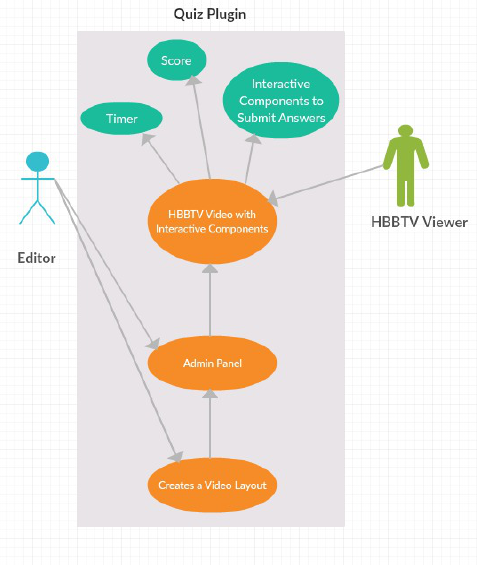
\includegraphics[scale=0.6]{figures/Use-case-Diagram.png}\\
	\caption{Use case Diagram }
	\label{fig:Use-case-Diagram}
\end{figure}
 
After that administrator’s responsibility will be to login to
admin panel and fill the details about questions. In the admin
panel, first of all, the admin will enter the question number,
which is just a sequence number of question in the database.
It has no effect on triggering events on screen. Secondly, the
admin will enter the start time of the question according to
the video, the end time of the question. These timestamps
will be responsible for triggering events on the screen such
as showing buttons to submit answers and these buttons will
disappear when question time expires. In the last section of this
form, the admin will enter the score for and correct answer for
that question. This information will verify the correct answer
to the question and updates the score accordingly.
 
    
   

 Figure \ref{fig:Admin-panel}.

\begin{figure}[!ht]
	\centering
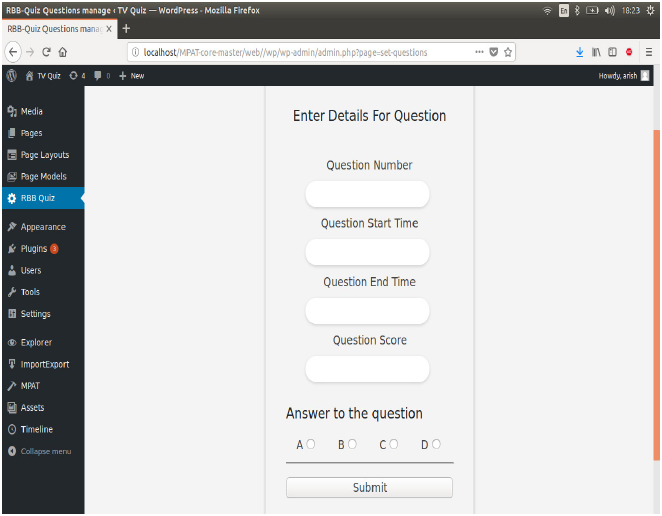
\includegraphics[scale=0.6]{figures/Admin-panel.png}\\
	\caption{Admin Panel}
	\label{fig:Admin-panel}
\end{figure} 
    
    
    
    
    
    
    
    
    
    
    

    
    
    

\subsection{TV User Interface}

When the video starts streaming, the HbbTV plugin will
populate the TV screen with different components. Following
are the components with their details: Figure \ref{fig:User-interface}.


    
    \begin{itemize}
       \item Timer Component
\item Score Component
\item Buttons to Submit Answer
    \end{itemize}




\begin{figure}[!ht]
	\centering
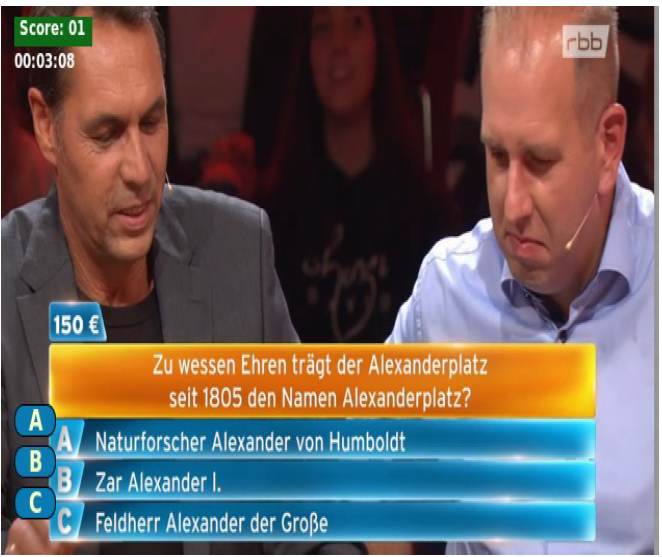
\includegraphics[scale=0.6]{figures/User-interface.png}\\
	\caption{User interface}
	\label{fig:User-interface}
\end{figure}




 \begin{enumerate}
 \item  Timer Component: 
 
 Timer component will show the current time on the video,
timer value will also be used to show answer components on
the score. When the time on time counter will be the same as
the time mentioned as the start time of question. Then exactly
on that time new components will appear on screen, where the
user can make the decision and selects the answer by the given
time for the question by the administrator of the show. For
each question, there is a start time and end time. In between
that time user has to make the decision and select any of the
possible answers.
 \item  Score Component: 
 
 Score component will always be there on the screen, but
it will update scores only when the video reaches at the end
time of each question. Total scores will be updated after every
question. The total core is dependent on the weights that the
administrator provides for each answer. The scoring algorithm
simply counts the weight of submitted answer and then adds
it to the current score value. If the user does not select any
answer the score will be zero. Once the user selects the answer
it will be locked and the right answer will appear after the
expiry of question time.
 \item  Buttons to Submit Answer:
 
 When TV host will announce the question in the Jede
Antwort zhlt, on the users screen three clickable buttons will
appear and these buttons will stay on screen until the question
time expires. User will only be able to select the answer only
once, and it will be locked until the right answer will be
revealed in the show. When the answer will be revealed the
player’s score will be updated in the core component.
Once the user selects the answer the color of the selected
answer will be changed and its locked. User will not be able
to change the answer once it is selected.
\end{enumerate}

 